\chapter{Árboles Binario de Búsqueda}
Un \textbf{Árbol Binario de Búsqueda} o \textbf{ABB} es aquel que los nodos del subárbol izquierdo contiene elementos menores a su padre y el subárbol derecho contiene elementos mayores a su padre (\textit{Figura 4.1: Representación de un árbol binario de búsqueda}).

Es importante saber que no pueden haber valores repetidos en este tipo de árboles, debido a que si no, no podremos comparar si esos elementos son menores o mayores (estrictos).

\begin{figure}[h]
  \begin{center}
    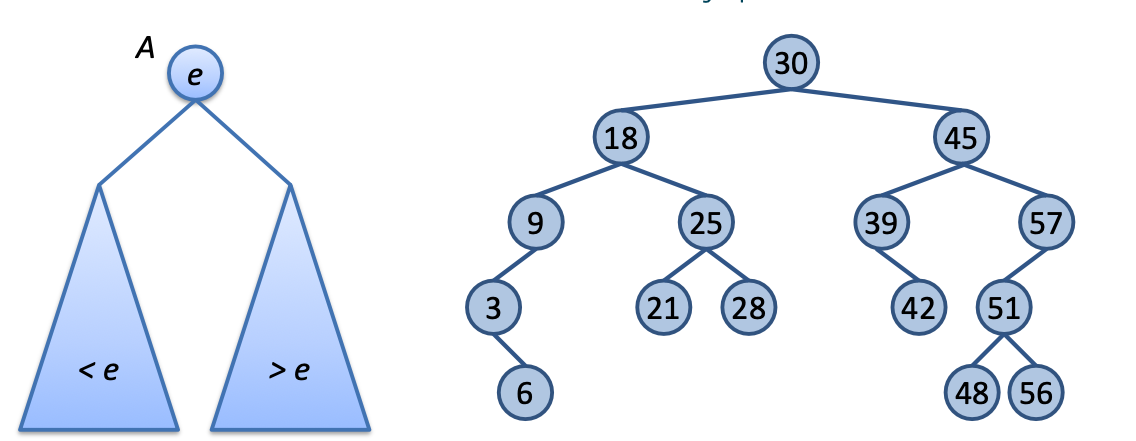
\includegraphics[width=0.7\textwidth]{assets/ABB1.png}
  \end{center}
  \caption{Representación de un árbol binario de búsqueda}
  Vemos que para un elemento `e' (18), el subárbol izquierdo va a contener elementos menores a él (9,3,6) y el derecho elementos mayores (25,21,28).
\end{figure}

Ahora, al saber que vamos a tener elementos `ordenados' por su valor a la hora de buscar un elemento en el árbol pasamos de un coste \textbf{\(O(n)\)} a un coste \textbf{\(O(log_{2}\ n)\)} debido a que al buscar un elemento (comparando si es mayor o menor que el padre) nos quitamos todo el subárbol que no cumple esa condición, es decir, o vamos por el hijo izquierdo o por el hijo derecho de ese padre, por los dos no.

\section{Ejemplo de búsqueda de un elemento en un ABB}
\begin{figure}[h]
  \hspace{-0.5cm}
  \begin{minipage}{.45\textwidth}
    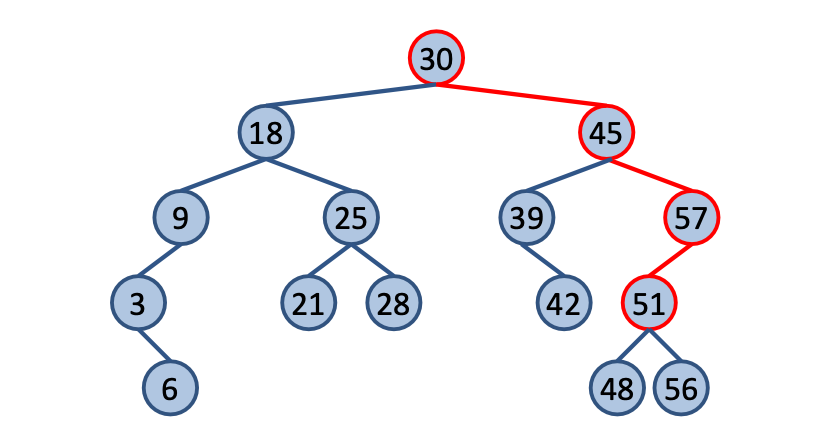
\includegraphics[width=\textwidth]{assets/Abb2.png}
  \end{minipage}
  \hspace{-0.5cm}
  \begin{minipage}{.5\textwidth}
  Queremos buscar el nodo cuyo elemento es `51', para ello hacemos:\\
  51 $>$ 30 → Hijo derecho de 30 → subárbol derecho\\
  51 $>$ 45 → Hijo derecho de 45 → subárbol derecho\\
  51 $<$ 57 → Hijo izquierdo de 57 → subárbol izquierdo\\
  51 $=$ 51 → hemos encontrado el nodo cuyo elemento es 51.
  \end{minipage}
\end{figure}
\newpage
\begin{minipage}{0.75\textwidth}
  Es importante saber que el tiempo de búsqueda depende de la estructura de ramificación del propio árbol. En este ejemplo, vemos que es un coste de \(O(log_{2}\ n)\), pero se puede dar el caso que el ABB es una lista de elementos por tanto, el coste sería \(O(n)\).
  \\

  En este caso, vemos que tenemos un árbol cuya ramificación se asemeja a una lista de elementos, por tanto, al no poder descartar ningún subárbol a la hora de buscar (por ejemplo el nodo con elemento 18) tendremos que recorrer toda la rama hasta llegar a ese nodo.
\end{minipage}
\vspace*{-5cm}
\begin{figure}[h]
  \begin{center}
    \hspace*{11.5cm}
    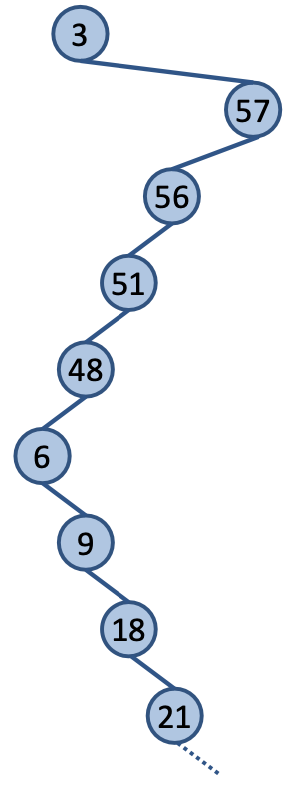
\includegraphics[width=.15\textwidth]{assets/abb3.png}
  \end{center}
  \caption{Ejemplo de ABB de coste \(O(n)\)}.
\end{figure}

\section{Especificación del TAD árbol binario de búsqueda}
Anteriormente, tanto en los árboles binarios como generales trabajábamos con nodos. Ahora en los árboles binarios de búsqueda vamos a trabajar con subárboles dependiendo de un valor `e'.

\subsection*{Constructor del árbol binario de búsqueda}
\underbar{\textit{Postcondición:}} Crea y devuelve un ABB vacío.\\
\verb|  Abb();|
\subsection*{Inserción de elementos en el ABB}
\underbar{\textit{Postcondición:}} Si `e' no pertence al árbol, lo inserta, en caso contrario el árbol no se modifica.\\
\verb|  void insertar(const T& e);| 
\subsection*{Eliminación de elementos del ABB}
\underbar{\textit{Postcondición:}} Si `e' se encuentra en el árbol, lo elimina, en caso contrario, el árbol no se modifica.\\
\verb|  void eliminar(const T& e);|
\subsection*{Métodos observadores de un ABB}
\begin{itemize}
  \item \underbar{\large\textbf{Obtener el subárbol}}:\\
  \underbar{\textit{Postcondición:}} Si `e' pertence al árbol devuelve el subárbol (cuya raíz es `e'), si no, devuelve un subárbol vacío.\\
  \verb|  const Abb& buscar(const T& e)const;|
  \item \underbar{\large\textbf{Estado vacío}}:\\ 
  \underbar{\textit{Postcondición:}} Devuelve \texttt{True} si el árbol está vacío, si no, \texttt{False}.\\
  \verb|  bool vacio()const;|
  \item \underbar{\large\textbf{Obtener subárbol izquierdo}}:\\
  \underbar{\textit{Precondición:}} Árbol no vacío.\\
  \underbar{\textit{Postcondición:}} Devuelve el subárbol izquierdo.\\
  \verb|  const Abb& izqdo()const;|
  \item \underbar{\large\textbf{Obtener subárbol derecho}}:\\
  \underbar{\textit{Precondición:}} Árbol no vacío.\\
  \underbar{\textit{Postcondición:}} Devuelve el subárbol derecho.\\
  \verb|  const Abb& drcho()const;|
\end{itemize}
\section{Implementación del TAD árbol binario de búsqueda}
\subsection{Implementación de un ABB mediante una estructura dinámica recursiva}
\begin{figure}[h]
  \begin{center}
    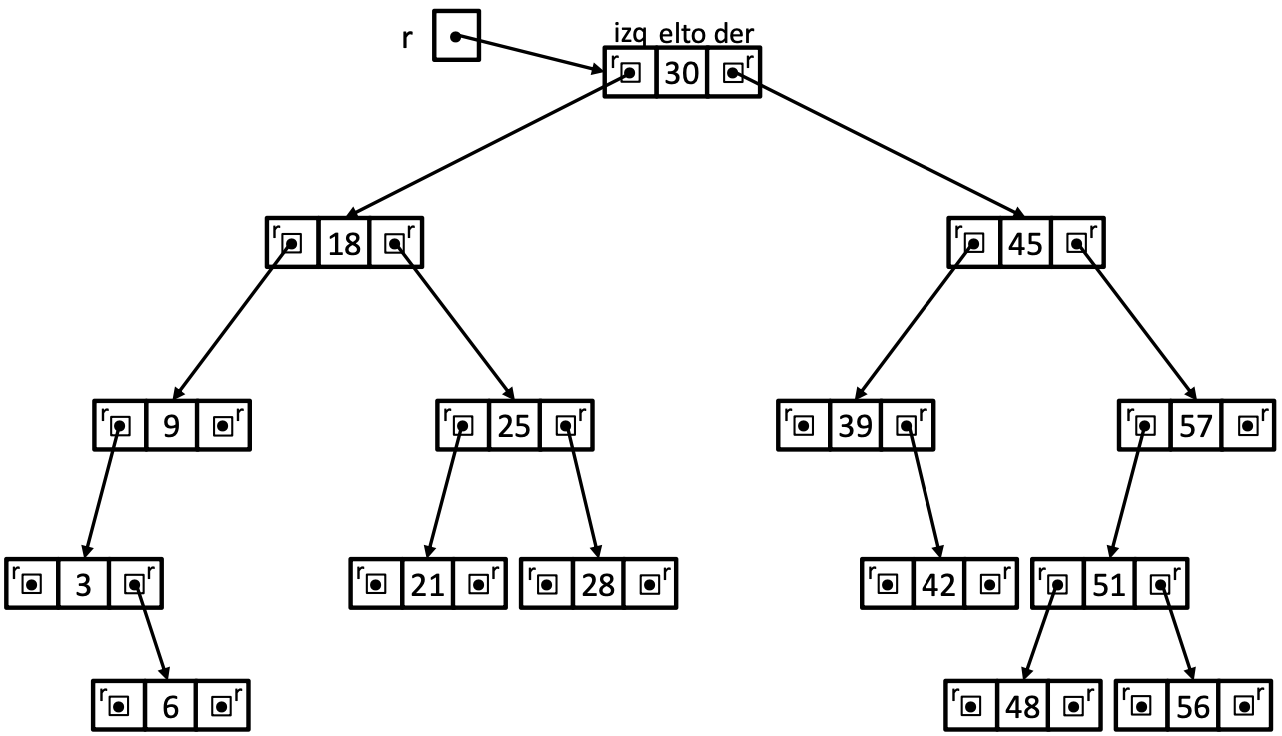
\includegraphics[width=0.6\textwidth]{assets/abb4.png}
  \end{center}
  \caption{Representación de la implementación dinámica recursiva}
\end{figure}

Vamos a hacer uso de esta implementación debido a que el método más `importante' de este TAD es el método \texttt{buscar()} (que nos devuelve el subárbol donde el elemento `e' es la raíz). Este método se realiza mediante llamadas recursiva y veremos como lo hace.

En la parte privada de TAD vamos a tener que almacenar el elemento y los dos subárboles (izquierdo y derecho).
\begin{minted}[breaklines]{C++}
template <typename T> class Abb{
  public:
    //Métodos vistos en la especificación del TAD
  private:
    struct arbol{
      T elto; //elemento
      Abb izq, der; //subárboles
      arbol(const T& e):elto(e),izq{},der{} {}
    };
    arbol *r;
};
\end{minted}
\subsubsection*{Implementación de la obtención del subárbol}
Ahora, vamos a ver como se implementa y que hace el método \texttt{buscar()}, mencionado anteriormente.
\begin{minted}[breaklines]{C++}
template <typename T>
const Abb<T>& Abb<T>::buscar(const T& e)const{
  if(r == nullptr)
    return *this; //Árbol vacio, no existe elemento
  else if(e < r->elto) //si es menor que el de la raiz, subárbol izquierdo
    return r->izq.buscar(e);
  else if(r->elto < e) //si es mayor, subárbol derecho
    return r->der.buscar(e);
  else 
    return *this; //encontrado en la raiz
}
\end{minted}

\subsubsection*{Inserción de un elemento en un ABB}
\begin{figure}[h]
  \begin{minipage}{0.4\textwidth}
    \vspace*{-2cm}
    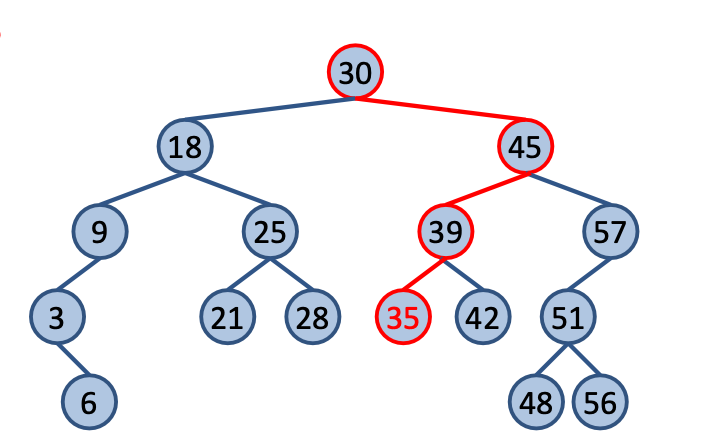
\includegraphics[width=\textwidth]{assets/abb5.png}
  \end{minipage}
  \hfill
  \begin{minipage}{0.5\textwidth}
    \begin{minted}[breaklines]{C++}
template <typename T>
void Abb<T>::insertar(const T& e){
  if(r==nullptr) //árbol vacio
      r = new arbol(e);
//se inserta en el subárbol izq.
  else if(e < r->elto) 
      r->izq.insertar(e);
//se inserta en el subárbol drch.
  else if(r->elto < e)
      r->der.insertar(e);
}
    \end{minted}
  \end{minipage}
\end{figure}

\underbar{\large\textbf{Ejemplo:}} Queremos insertar en el árbol anterior el elemento `35' (indicado en rojo),\\para ello la traza a seguir (según el código dado) sería:
\\
\hspace*{1cm}35 $>$ 30 → Hijo derecho de 30 → subárbol derecho.\\
\hspace*{1cm}35 $<$ 45 → Hijo izquierdo de 45 → subárbol izquierdo.\\
\hspace*{1cm}35 $<$ 39 → Hijo izquierdo de 39 → subárbol izquierdo.\\

Como el nodo cuyo valor es `39' no tiene subárbol izquierdo y 35 es menor que él, insertamos dicho valor como `hijo izquierdo' del nodo con valor 39.

\textit{NOTA}: Si encontramos que dicho valor ya se encuentra en el árbol no hacemos nada, ya que no podemos tener valores repetidos en el árbol.
\newpage
\subsubsection*{Eliminación de un elemento en un ABB}
A la hora de eliminar un elemento de un ABB no tenemos como precondición que el nodo que contiene a ese elemento sea una hoja, por tanto, encontramos 3 casos(cuando es hoja, tiene un hijo y tiene ambos hijos):

\begin{itemize}
  \item \textbf{Caso 1: Eliminación de un nodo hoja:}
  
    \begin{minipage}{0.4\textwidth}
      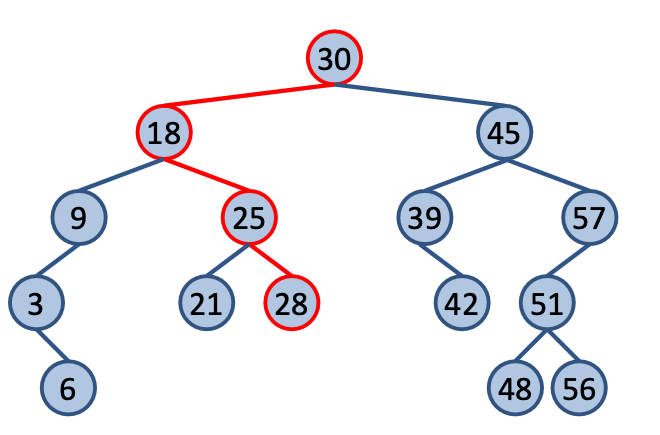
\includegraphics[width=\textwidth]{assets/abb6.png}
    \end{minipage}
    \hfill
    \begin{minipage}{0.5\textwidth}
    Queremos eliminar el nodo con elemento `28'(indicado en rojo), para ello:
    \\
    28 $<$ 30 → Hijo izquierdo de 30 → subárbol izquierdo.\\
    18 $<$ 28 → Hijo derecho de 18 → subárbol derecho.\\
    25 $<$ 28 → Hijo derecho de 25 → subárbol derecho.\\
    Como 28 = 28, lo eliminamos.
    \end{minipage}
    \underbar{Como resultado quedaría:}
  \begin{center}
    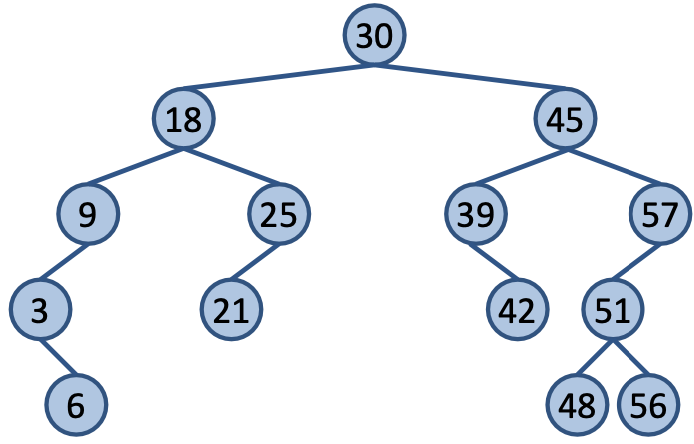
\includegraphics[width=.4\textwidth]{assets/abb11.png}
  \end{center}
  \item \textbf{Caso 2: Eliminación de un nodo con un hijo:}\\
  Este caso es un poco diferente, ya que el nodo a eliminar va a tener o hijo izquierdo o derecho.\\
  \begin{minipage}{0.4\textwidth}
    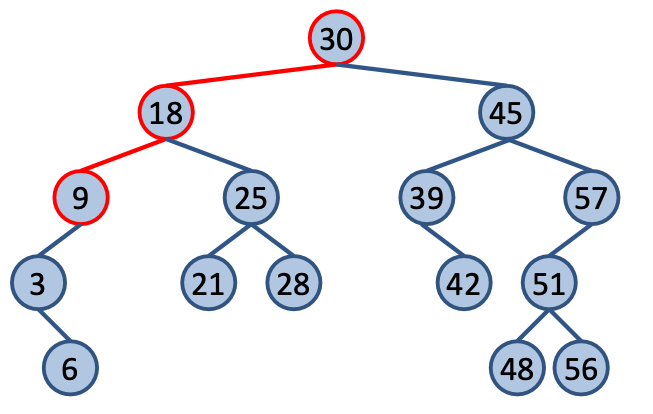
\includegraphics[width=\textwidth]{assets/abb7.png}
  \end{minipage}
  \hfill
  \begin{minipage}{0.5\textwidth}
  Queremos eliminar el nodo con elemento `9'(indicado en rojo), para ello:
  \\
  9 $<$ 30 → Hijo izquierdo de 30 → subárbol izquierdo.\\
  9 $<$ 18 → Hijo derecho de 18 → subárbol derecho.\\
  Como 9 = 9, lo eliminamos y su hijo pasa a ser el nuevo hijo izquierdo del `padre de 9', es decir el nodo con valor `18'.
  \end{minipage}

  \underbar{Como resultado quedaría:}
  \begin{center}
    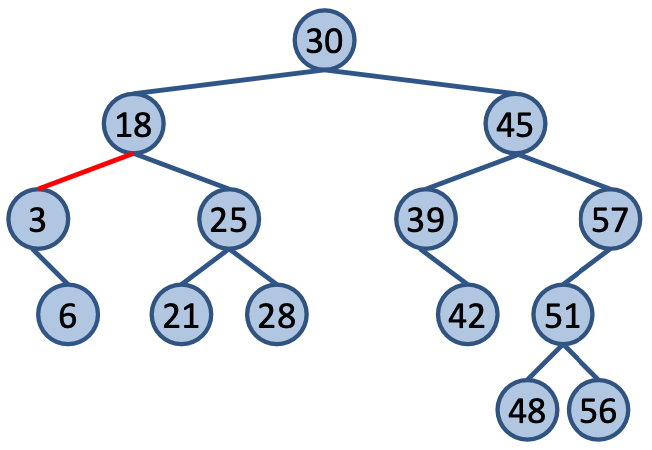
\includegraphics[width=.4\textwidth]{assets/abb10.png}
  \end{center}
  \newpage

  \item \textbf{Caso 3: Eliminación de un nodo con ambos hijos:}
  
  Este caso es parecido al caso 2, con la única diferencia que ahora el nodo a eliminar tiene tanto hijo izquierdo como derecho. Esto se soluciona buscando a los candidatos para ocupar su posición en el árbol, estos pueden ser el \textbf{mayor elemento del subárbol izquierdo} o el \textbf{menor elemento del subárbol derecho}.

  \begin{minipage}{0.4\textwidth}
    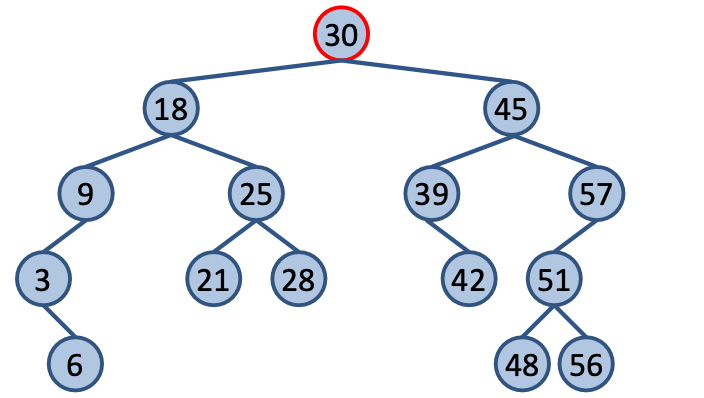
\includegraphics[width=\textwidth]{assets/abb8.png}
  \end{minipage}
  \hfill
  \begin{minipage}{0.5\textwidth}
  Como vemos, queremos eliminar el nodo con valor `30' (tiene dos hijos 18 y 45). Por tanto, los candidatos válidos son el nodo con mayor valor del subárbol que tiene como raíz `18' ó el nodo con menor valor del subárbol que tiene como raíz `45'.

  Hemos escogido el nodo con menor valor del subárbol derecho que es `39', pero este tiene un hijo derecho `42' que pasará a ser hijo izquierdo del nodo con valor `45'.
  \end{minipage}
  \underbar{Como resultado quedaría:}
  \begin{center}
    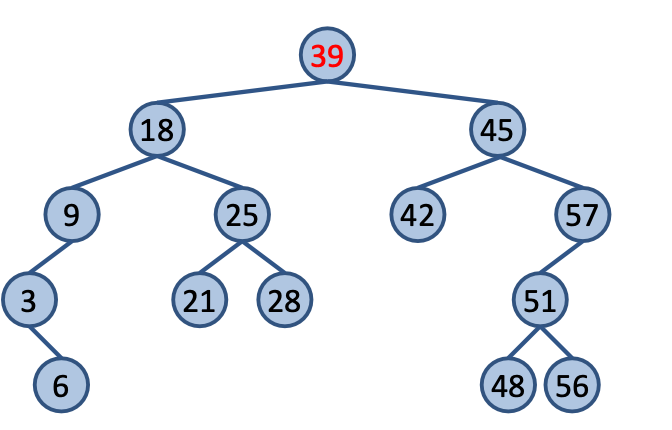
\includegraphics[width=.4\textwidth]{assets/abb9.png}
  \end{center}
\end{itemize}

\textbf{Código de la eliminación de elementos de un ABB:}
\begin{minted}[breaklines]{C++}
template <typename T> void Abb<T>::eliminar(const T& e){
  if(r!=nullptr){ //Caso 1: es hoja
    if(e < r->elto)
      r->izq.eliminar(e);
    else if(r->elto < e)
      r->der.eliminar(e);
  }
  else if(!r->izq.r && !r->der.r) //raíz es hoja
    delete r;
    r == nullptr;
  else if(!r->der.r) //Caso 2: Solo tiene un hijo (izquierdo)
    arbol *a = r->izq.r;
    r->izq.r = nullptr;
    delete r;
    r = a;
  else if(!r->izq.r) //Caso 2: Ánalogo para el derecho
    arbol *a = r->der.r;
    r->der.r = nullptr;
    delete r;
    r = a;
  else //Caso 3: Tiene ambos hijos
    r->elto = r->der.borrarMin();
}
\end{minted}



